\documentclass[border=10pt]{standalone}
\usepackage{pgfplots}
\pgfplotsset{compat=1.18}

\begin{document}

% xy-trace (z=0)
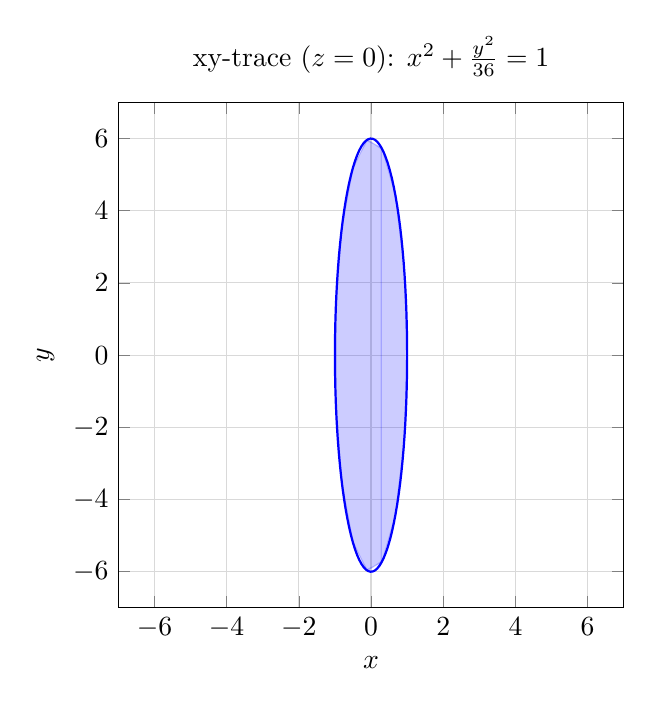
\begin{tikzpicture}
\begin{axis}[
    xlabel={$x$},
    ylabel={$y$},
    title={xy-trace ($z=0$): $x^2 + \frac{y^2}{36} = 1$},
    axis equal,
    grid=both,
    grid style={gray!30},
    width=8cm,
    height=8cm,
    xmin=-1.5, xmax=1.5,
    ymin=-7, ymax=7,
]
\addplot[blue, thick, domain=0:2*pi, samples=100] 
    ({cos(deg(x))}, {6*sin(deg(x))});
\addplot[blue, fill, opacity=0.2] 
    ({cos(deg(x))}, {6*sin(deg(x))}) -- cycle;
\end{axis}
\end{tikzpicture}

\end{document}